% !TEX root = main.tex

\section{Introduction}

\noindent Heterogeneous systems composed of latency optimized cores
(e.g. CPUs) and throughput optimized cores (e.g. GPUs, MIC~\cite{MIC})
are becoming the defacto organization of future high performance
computing platforms. Such systems typically consist of a hybrid memory
system~\cite{hbm_intel,hbm_amd,hbm_nvidia} that is composed of
commodity DRAM~\cite{ddr4-spec} and stacked
DRAM~\cite{hbm-spec,hmc_spec}. Furthermore, such systems also support
{\em Shared Virtual Memory}~\cite{HSA,UVM} where both CPUs and GPUs
access the entire hybrid memory address space using a unified virtual
address space.
%Consequently, the performance of
%emerging heterogeneous systems is dependent on hardware support for
%virtual memory.

In the virtual memory framework, depending on the page table
implementation, address translation requires one or more page table
accesses~\cite{Bhargava2008}. To avoid the long memory access latency,
processor architects cache recent address translations using an
on-chip multi-level translation look-aside buffer (TLB) hierarchy.
Growing application working-set sizes continue to stress the on-chip
{\em Last-Level TLB (LLT)}~\cite{spectlb, Basu2013, SharedLLT, COLT}.
LLT misses are latency sensitive operations that require one or more
serial accesses to the page table. Therefore, virtual memory
performance is dependent on the performance of the LLT. Reducing LLT
miss latency enables instructions depending on the missing TLB entry
to make faster forward progress.

A recent real system measurement study shows significant opportunity
to improve shared virtual memory performance of heterogeneous CPU-GPU
systems~\cite{vesley2016ispass}. Specifically, they show that LLT
misses are an order of magnitude slower on the GPU relative to the
CPU. Thus, we focus on improving GPU LLT miss overhead in CPU-GPU
systems by reducing both LLT miss {\em frequency} and LLT miss {\em
latency}.

% with a heterogeneous memory system\footnote{Heterogeneous memory
% systems are designed since stacked DRAM cannot completely replace
% DDR~\cite{BEAR,moin2012}}.
%Since page tables are
%conventionally stored in commodity DRAM (here on referred to as system
%memory), frequent LLT misses degrade performance due to the long queuing delays
%in the memory subsystem. 


\begin{figure}[t] 
\vspace{-0.2 in}
\centering
\centerline{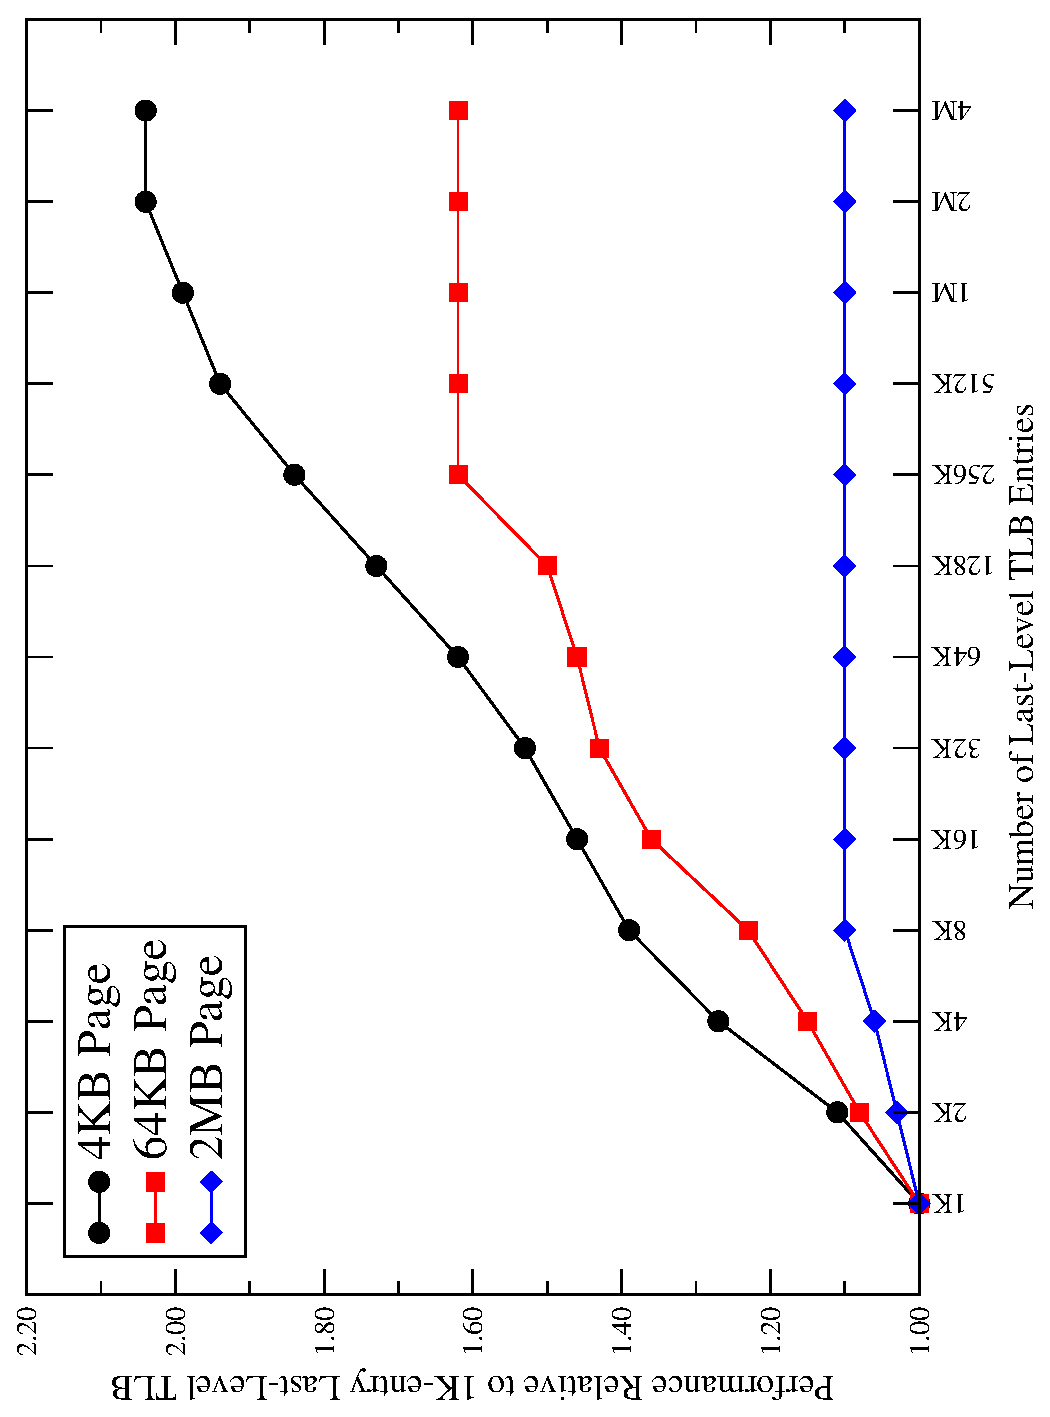
\psfig{file=GRAPHS/tlb_sensitivity,angle=-90,width=\columnwidth}}

	\caption{\small Performance Sensitivity to LLT Entries. \normalsize}

\label{fig:tlb_sensitivity} 
\vspace{-0.15 in}
\end{figure}

A simple solution to reduce LLT miss frequency would be to increase
LLT size to cover the application working-set size.
Figure~\ref{fig:tlb_sensitivity} shows GPU performance sensitivity to
LLT size relative to a 1024-entry shared
LLT\footnote{Section~\ref{sec:method} discusses workloads and
simulation methodology.}. The x-axis shows TLB sizes, while the y-axis
shows average performance relative to the baseline for three different
page sizes: 4KB, 64KB, and 2MB. The figure shows that performance is
highly sensitive to the number of LLT entries with smaller page sizes.
On average, a two million entry LLT improves performance by 2X with a
4KB page size. Similarly, a 256k-entry LLT improves performance by
60\% with 64KB page size. Finally, an 8k-entry LLT improves
performance by 10\% with 2MB page size. Note that as application
memory working-set size grow larger, the performance sensitivity to
larger LLT size also increases with large page sizes.

%Assuming 8-bytes of storage requirement per TLB entry, processor
%architects would need to budge 16MB, 2MB, and 64KB of area overhead
%for 4KB, 64KB, and 2MB pages respectively. 

%This is because a single large page (e.g. 2MB) TLB entry can
%span hundreds of contiguous small page (e.g. 4KB) TLB entries. 
%Covering a larger portion of the virtual address space using
%entries of the on-chip multi-level TLB hierarhcy results in fewer page
%table accesses in memory and avoids long memory access latencies. 
Unfortunately, on-die area limitations prohibit simply increasing the
LLT size, especially with smaller page sizes. Recent work has
investigated improving performance of virtual memory translation using
large pages to help TLB coverage. However, unrestricted use of large
pages can create unintended OS performance overheads
~\cite{SuperPageProblem, TwoPageSize} due to memory
imbalance~\cite{numa-harmful}, memory fragmentation,
paging~\cite{cameo}, page creation, and page
splitting~\cite{largepagevm}. Consequently, the use of large pages
have traditionally been limited to complex server systems that have
their own run-time systems to manage memory (e.g. Oracle
DBMS~\cite{oracle_dbms}, SAP~\cite{sap}). As such, this paper focuses
on increasing on-die TLB coverage with small page sizes without high
storage overhead or changes to the existing virtual memory system.

We propose hardware mechanisms to improve LLT coverage and LLT miss
penalty. Our first mechanism, {\em Unified Cache and TLB (UCAT)},
reduces the frequency of on-die LLT misses by enabling the
conventional unified LLC to also hold TLB entries. UCAT augments the
existing on-die LLT and increases on-die TLB coverage by potentially
allowing as many TLB entries as there are cache lines in the
conventional on-chip LLC.

%entirely in software, proposes to allocate the frequently
%accessed portion of the application page table in stacked memory.
%Doing so significantly improves LLT miss latency compared to storing
%the entire page table in system memory. 

However, UCAT {\em does not} reduce the LLT miss penalty incurred from
walking the page table. This is because an LLT miss still requires
multiple long-latency, serial, accesses to the page table. To this
end, we propose {\em DRAM-TLB}, a hardware mechanism to memoize
virtual to physical translations in DRAM. DRAM-TLB serves as the next
larger TLB in the processor TLB hierarchy whose contents are identical
to the contents of on-chip TLBs. A DRAM-TLB is consulted upon LLT (or
UCAT) misses before walking the page table.

% (i.e. virtual and physical address pairs, permission
%bits, and address space identifier (ASID)). 

% The DRAM-TLB physically resides in memory and requires negligible
% storage overhead. Furthermore, they can be sized arbitrarily such that
% address translations can be retrieved with a single memory access.

Overall, this paper makes the following contributions:

\begin{enumerate}

  \item{We extend on-die TLB coverage by enabling the conventional LLC
    to serve as a {\em Unified Cache and TLB (UCAT)}. UCAT holds cache
    lines and TLB entries in a single hardware structure. Thus, UCAT
    improves on-die TLB coverage by enabling as many on-die TLB
    entries as there are cache lines in the conventional on-chip LLC.}

  \item{We reduce LLC miss penalty by architecting {\em TLBs in DRAM
    (DRAM-TLB)}. A DRAM-TLB is a very large hardware-managed structure
    that logically sits between the LLT (or UCAT) and the page table.
    A DRAM-TLB can be arbitrarily sized to provide the desired TLB
    coverage by only occupying a very small portion of gigantic DRAM
    sizes in today's systems. Unlike a page table walk, a DRAM-TLB
    provides low-latency address translation with a single memory
    access. }


  \item{We propose DUCATI, an address translation architecture that
  combines DRAM-TLB and UCAT benefits to improve TLB coverage and LLT
  miss latency in high performance computing systems.}

\end{enumerate}

\noindent For a set of high performance computing workloads simulated
on a heterogeneous CPU-GPU system with 4KB page size, Unified Cache
and TLB (UCAT) improves performance by 65\% on average (up to 4x). On
the other hand, DRAM-TLB improves performance by 22\% on average (up
to 2.25X). Both proposals combined, DUCATI, improves performance by
81\% (up to 4.5x). We also show that DUCATI requires negligible
hardware changes and scales to larger page sizes and improves
performance by 56\% and 8\% when using 64KB and 2MB pages
respectively.

%\item{To the best of our knowledge, this is the first study that
%leverages stacked memory to improve TLB miss overhead. While these
%proposals may seem obvious and incremental, the value is in their
%simplicity. Our proposals significantly improve TLB miss overhead
%without redesigning the existing address translation hardware.}

% \item{We propose {\em Stacked Memory Placement}, a software mechanism
%    that places the entire hierarchical page table in stacked memory.
%    Doing so improves LLT miss latency due to lower stacked memory
%    queuing delays.}

%\item{We propose a software mechanism, {\em Distributed Placement},
%   that reduces DRAM queuing delays by placing the frequently accessed
%   page table level in stacked memory and the remainder in system
%   memory.}

% \item{While high performing, we show that page table placement does
%   not reduce the bandwidth required for address translation. This is
%   because LLT misses still require multiple page table accesses for
%   address translation. To address this problem, we propose hardware
%   support to increase the TLB hierarchy by placing {\em TLBs in
%   DRAM}.}


% \item{We propose a hardware mechanism, {\em Stacked-TLB}, that embeds
%    a gigantic TLB in stacked memory. Stacked-TLB logically sits
%    between the LLT and the page table. Unlike a page table walk,
%    Stacked-TLB provides low-latency and low-bandwidth translations
%    since it incurs a single memory access. }

%  We place the DRAM-TLB in stacked memory and refer to it as {\em
%    Stacked-TLB}.

% We show that Stacked-TLB requires low storage overhead, is scalable,
% and can be configured to provide full TLB coverage for any
% application memory footprint.

% \item{We show that Stacked-TLB requires low storage overhead, is
%   scalable, and can be configured to provide full TLB coverage for any
%   application memory footprint.}

% address translation system.

\begin{figure}[bp] 
\vspace{-0. in}
\centering
 	\centerline{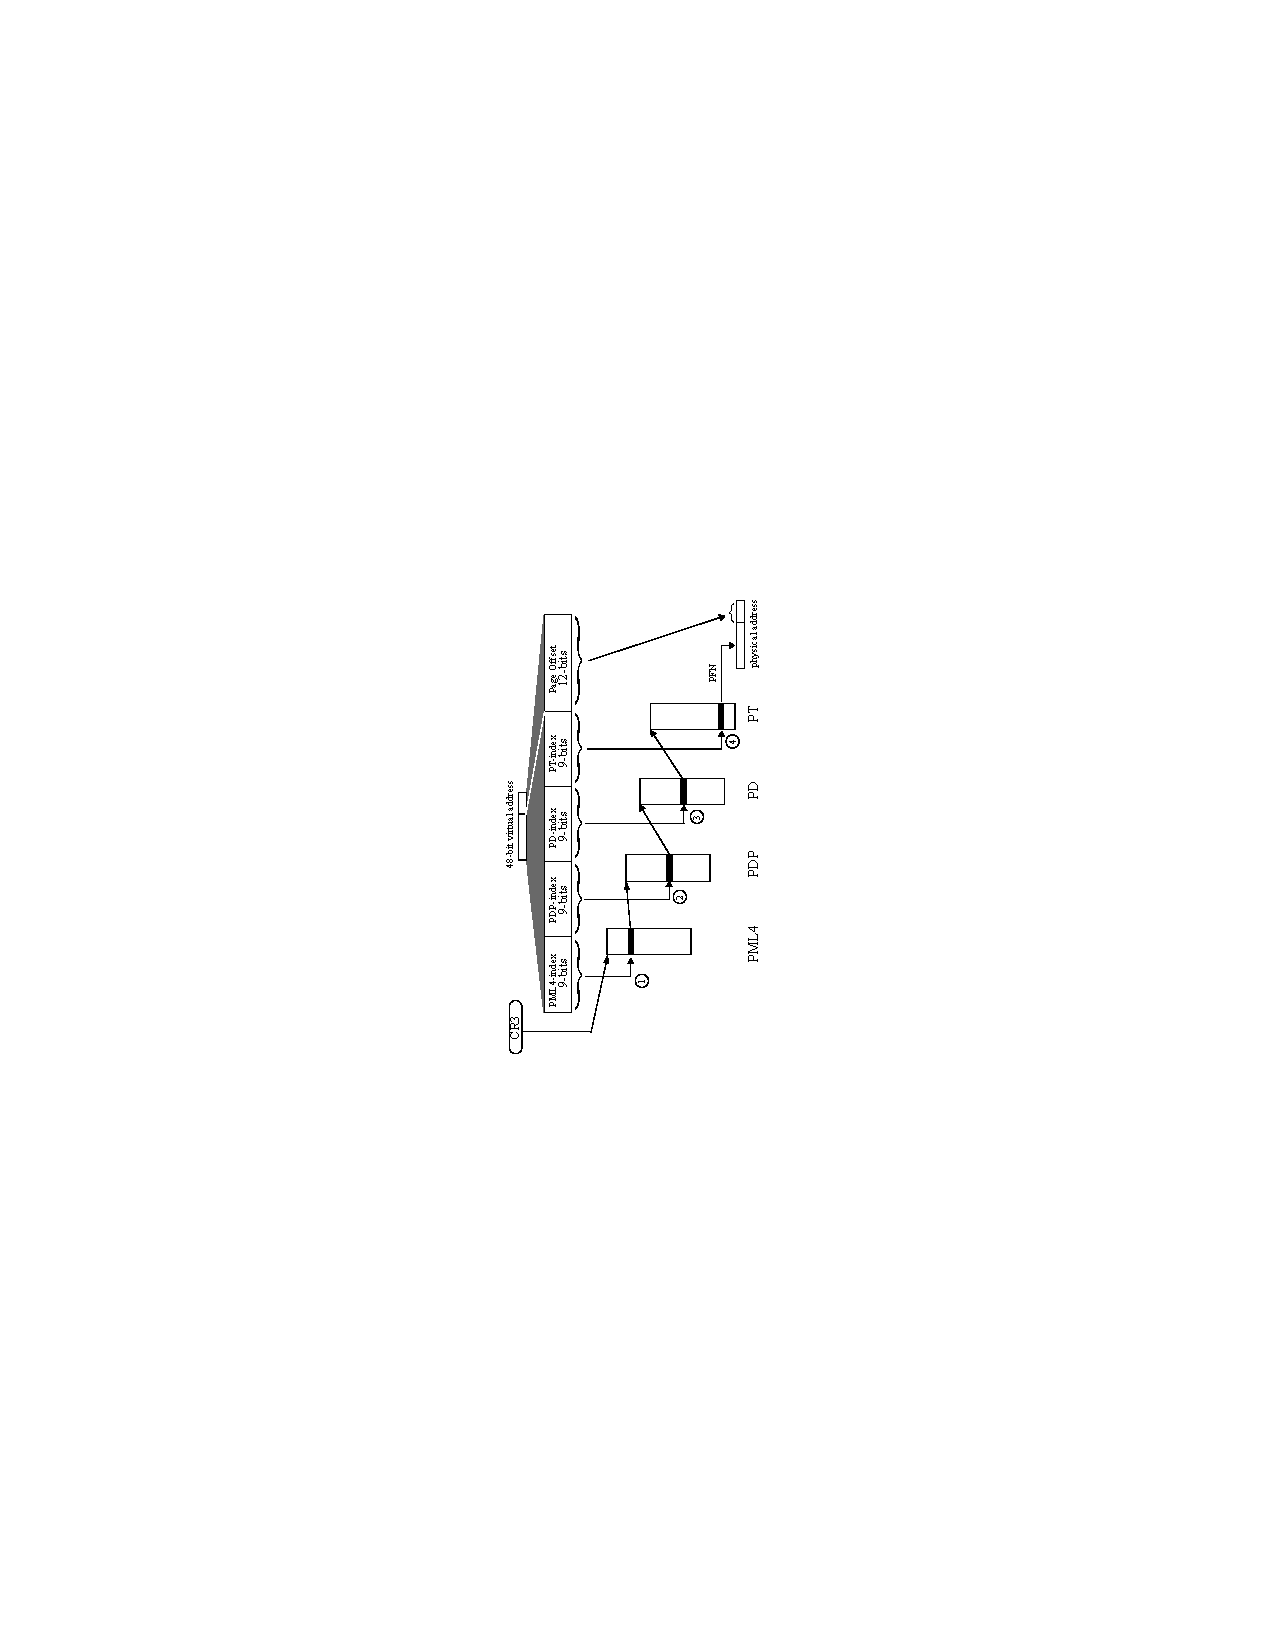
\psfig{file=FIGURES/page_table,angle=-90,width=\columnwidth}}
%	\centerline{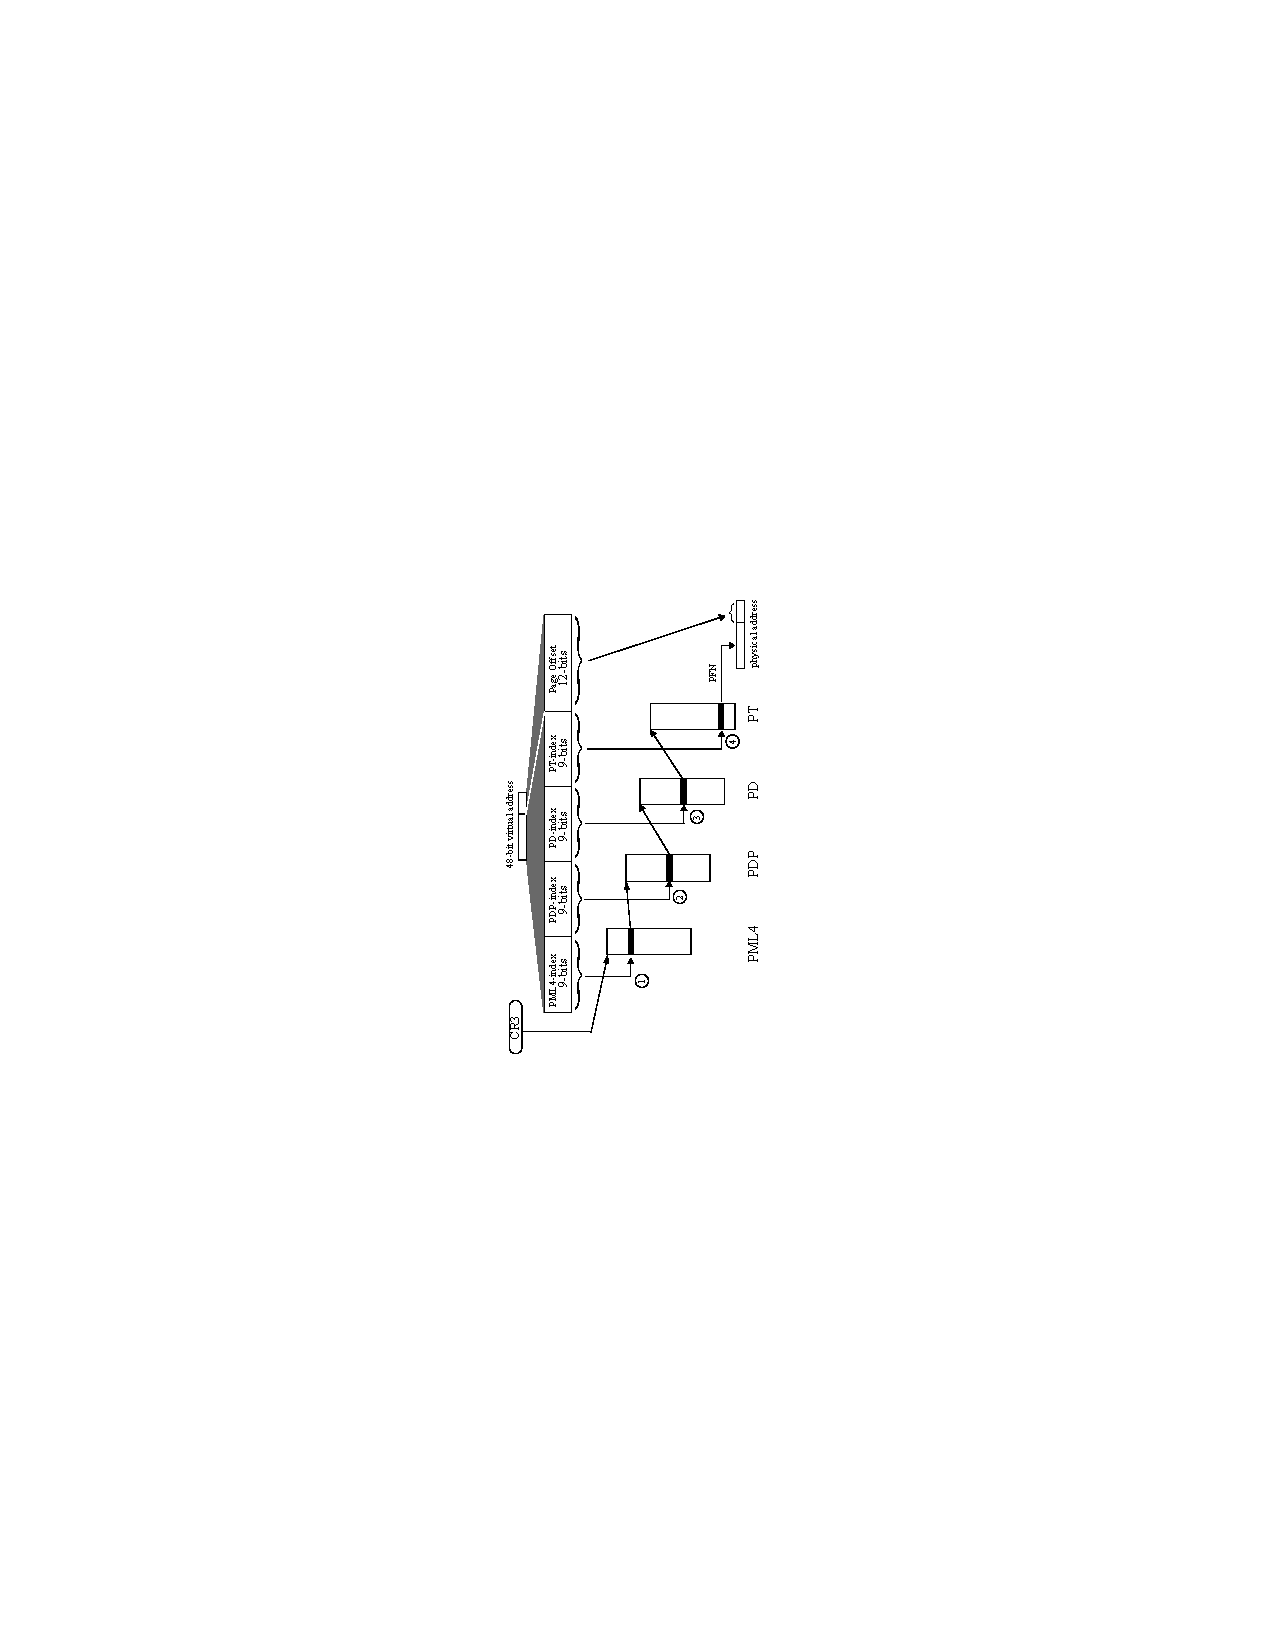
\psfig{file=FIGURES/page_table,angle=-90,width=\textwidth}}

	\caption{\small A four-level hierarchical page table.
	\normalsize}
\label{fig:page_table} 
\vspace{-0. in}
\end{figure}

%List of things that have been removed from the old intro that need to be 
%added either to the background section or perhaps related work if the 
%shortened version of them that comes in the intro above doesn't satisfy
%what needs to be communicated:

%the below used to be second paragraph. I think most of it is now 
%covered, but if we want some of this we can include it in background too.
%-------------
%Under the virtual memory framework, programs operate on virtual
%addresses that must be dynamically translated to physical addresses.
%The operating system (OS) maintains a {\em page table} in memory that
%maps application virtual addresses to physical addresses. Depending on
%the page table implementation, address translation requires one or
%more page table accesses~\cite{Bhargava2008}. To avoid the long memory
%access latency, processor architects cache recent address translations
%using an on-chip multi-level translation look-aside buffer (TLB)
%hierarchy. Therefore, virtual memory performance is dependent on the
%performance of the {\em Last-Level TLB (LLT)}.
%-------------

%the below used to be the fifth paragraph, seemed totally out of place
%so i commented it. It can be moved to related work:
%-------------
%Alternatively, TLB coverage can be improved through the use of direct
%segments~\cite{Basu2013}. While high performing, from a practical
%implementation perspective, direct segments require non-negligible
%hardware and software changes to the baseline address translation
%system. Furthermore, direct segments can also suffer from problems
%similar to those of large pages.
%-------------

%the below used to be the sixth paragraph, again should be moved to related
%work or mentioned in methodology if the goal is to explain that we have
% a good baseline:
%-------------
%Several studies have also focused on practical solutions to improve
%LLT performance. These proposals reorganize the TLB
%hierarchy~\cite{SharedLLT}, prefetch TLB entries
%~\cite{prefTLBintercore, prefTLBgokul, prefTLBrecency,
%power2014supporting}, speculate address translation on TLB
%misses~\cite{spectlb}, speed up page walks by caching page table
%entries~\cite{SkipPT, MMUcaches, power2014supporting}, or compress
%several translations into a single TLB entry~\cite{COLT}. Our
%evaluations with these techniques~\cite{SharedLLT, COLT, MMUcaches} in
%our baseline system show that there is still significant room to
%improve the performance overhead of LLT misses when using small pages.
%-------------





